%===============================================================================
\begin{figure*}[t]
	\centering
	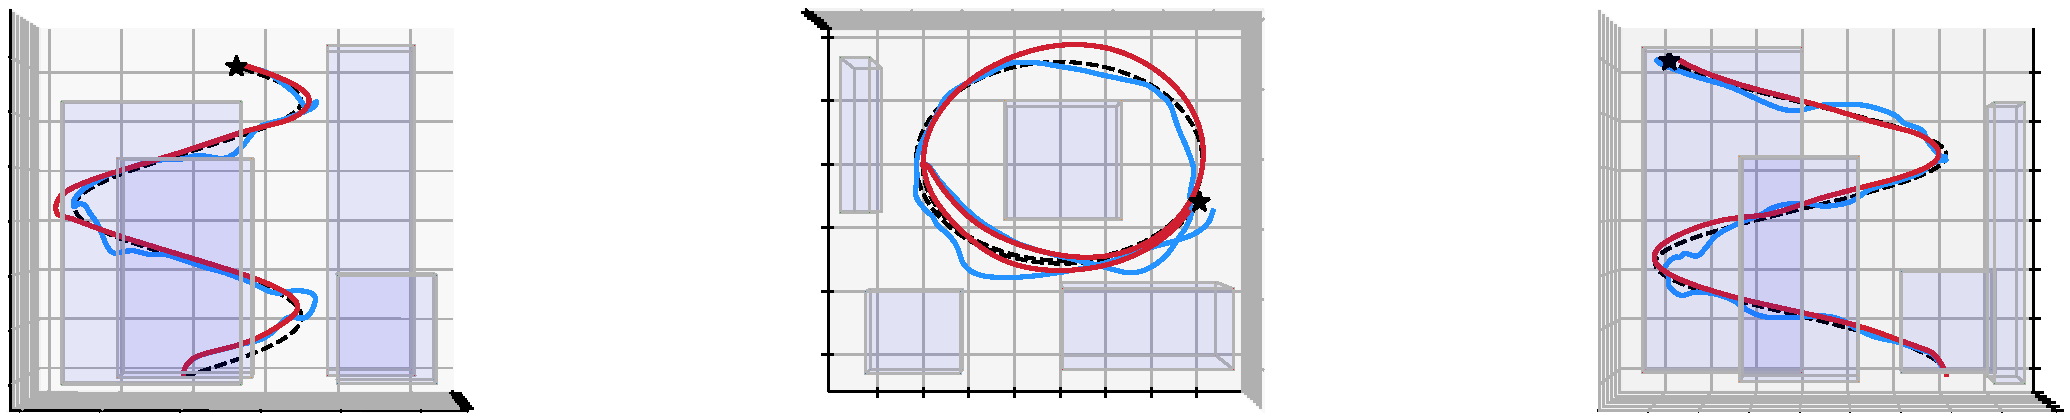
\includegraphics[width=\textwidth]{figures/plot_3D}
	\vspace{-0.5cm}
	\caption{Generated trajectories among obstacles (purple) using our mixed-initiative NMPC: novice pilot (blue); experienced pilot (red); reference trajectory is dashed; the $\star$ marks the final goal.}\label{fig:output}%
\end{figure*}
%===============================================================================
\begin{figure*}[t]
\centering
\subfloat[Novice.]{\includegraphics[width=0.5\textwidth]{figures/inputs_novice}} 
\subfloat[Experienced.]{\includegraphics[width=0.5\textwidth]{figures/inputs_experienced}}
\caption{Pilot inputs generated by an autonomous algorithm and mixed-initiative NMPC commands as a result of the blending mechanism.}\label{fig:human_inputs_s1}%
\end{figure*}
%===============================================================================

In real-time NMPC applications, Problem \ref{problem:mi} needs to be solved at each sampling instant under the available computation time. To that end, we use a numerical strategy based on sequential quadratic programming (SQP) that relies on the solution of a limited number of QP subproblems, the so-called real-time iteration (RTI) scheme \cite{diehl2005}. More precisely, only one linearization and QP solve are carried out per sampling instant, leading to an approximate feedback control policy. An essential element in the RTI scheme is to keep the initial state $\xi_0$ as a constrained decision variable, often referred to as \emph{initial value embedding}. This trait allows one to divide computations into a preparation and feedback phase, where the former is typically more expensive. In this work, we will be using the RTI method's implementation through the high-performance software package \texttt{acados} \cite{verschueren2019}. Through \texttt{acados} Python template-based interface, we generate the library that implements Problem \ref{problem:mi}, which is then wrapped by our framework written in Python. 